\section{Additional Diagnostic Figures}
\label{app:diagnostic_figures}

This appendix collects validated diagnostic figures that support the main Results figures without interrupting the paper body. The main paper keeps one figure per central claim; the appendix preserves denser synthesis and secondary evidence for auditability.

\begin{figure*}[t]
\centering
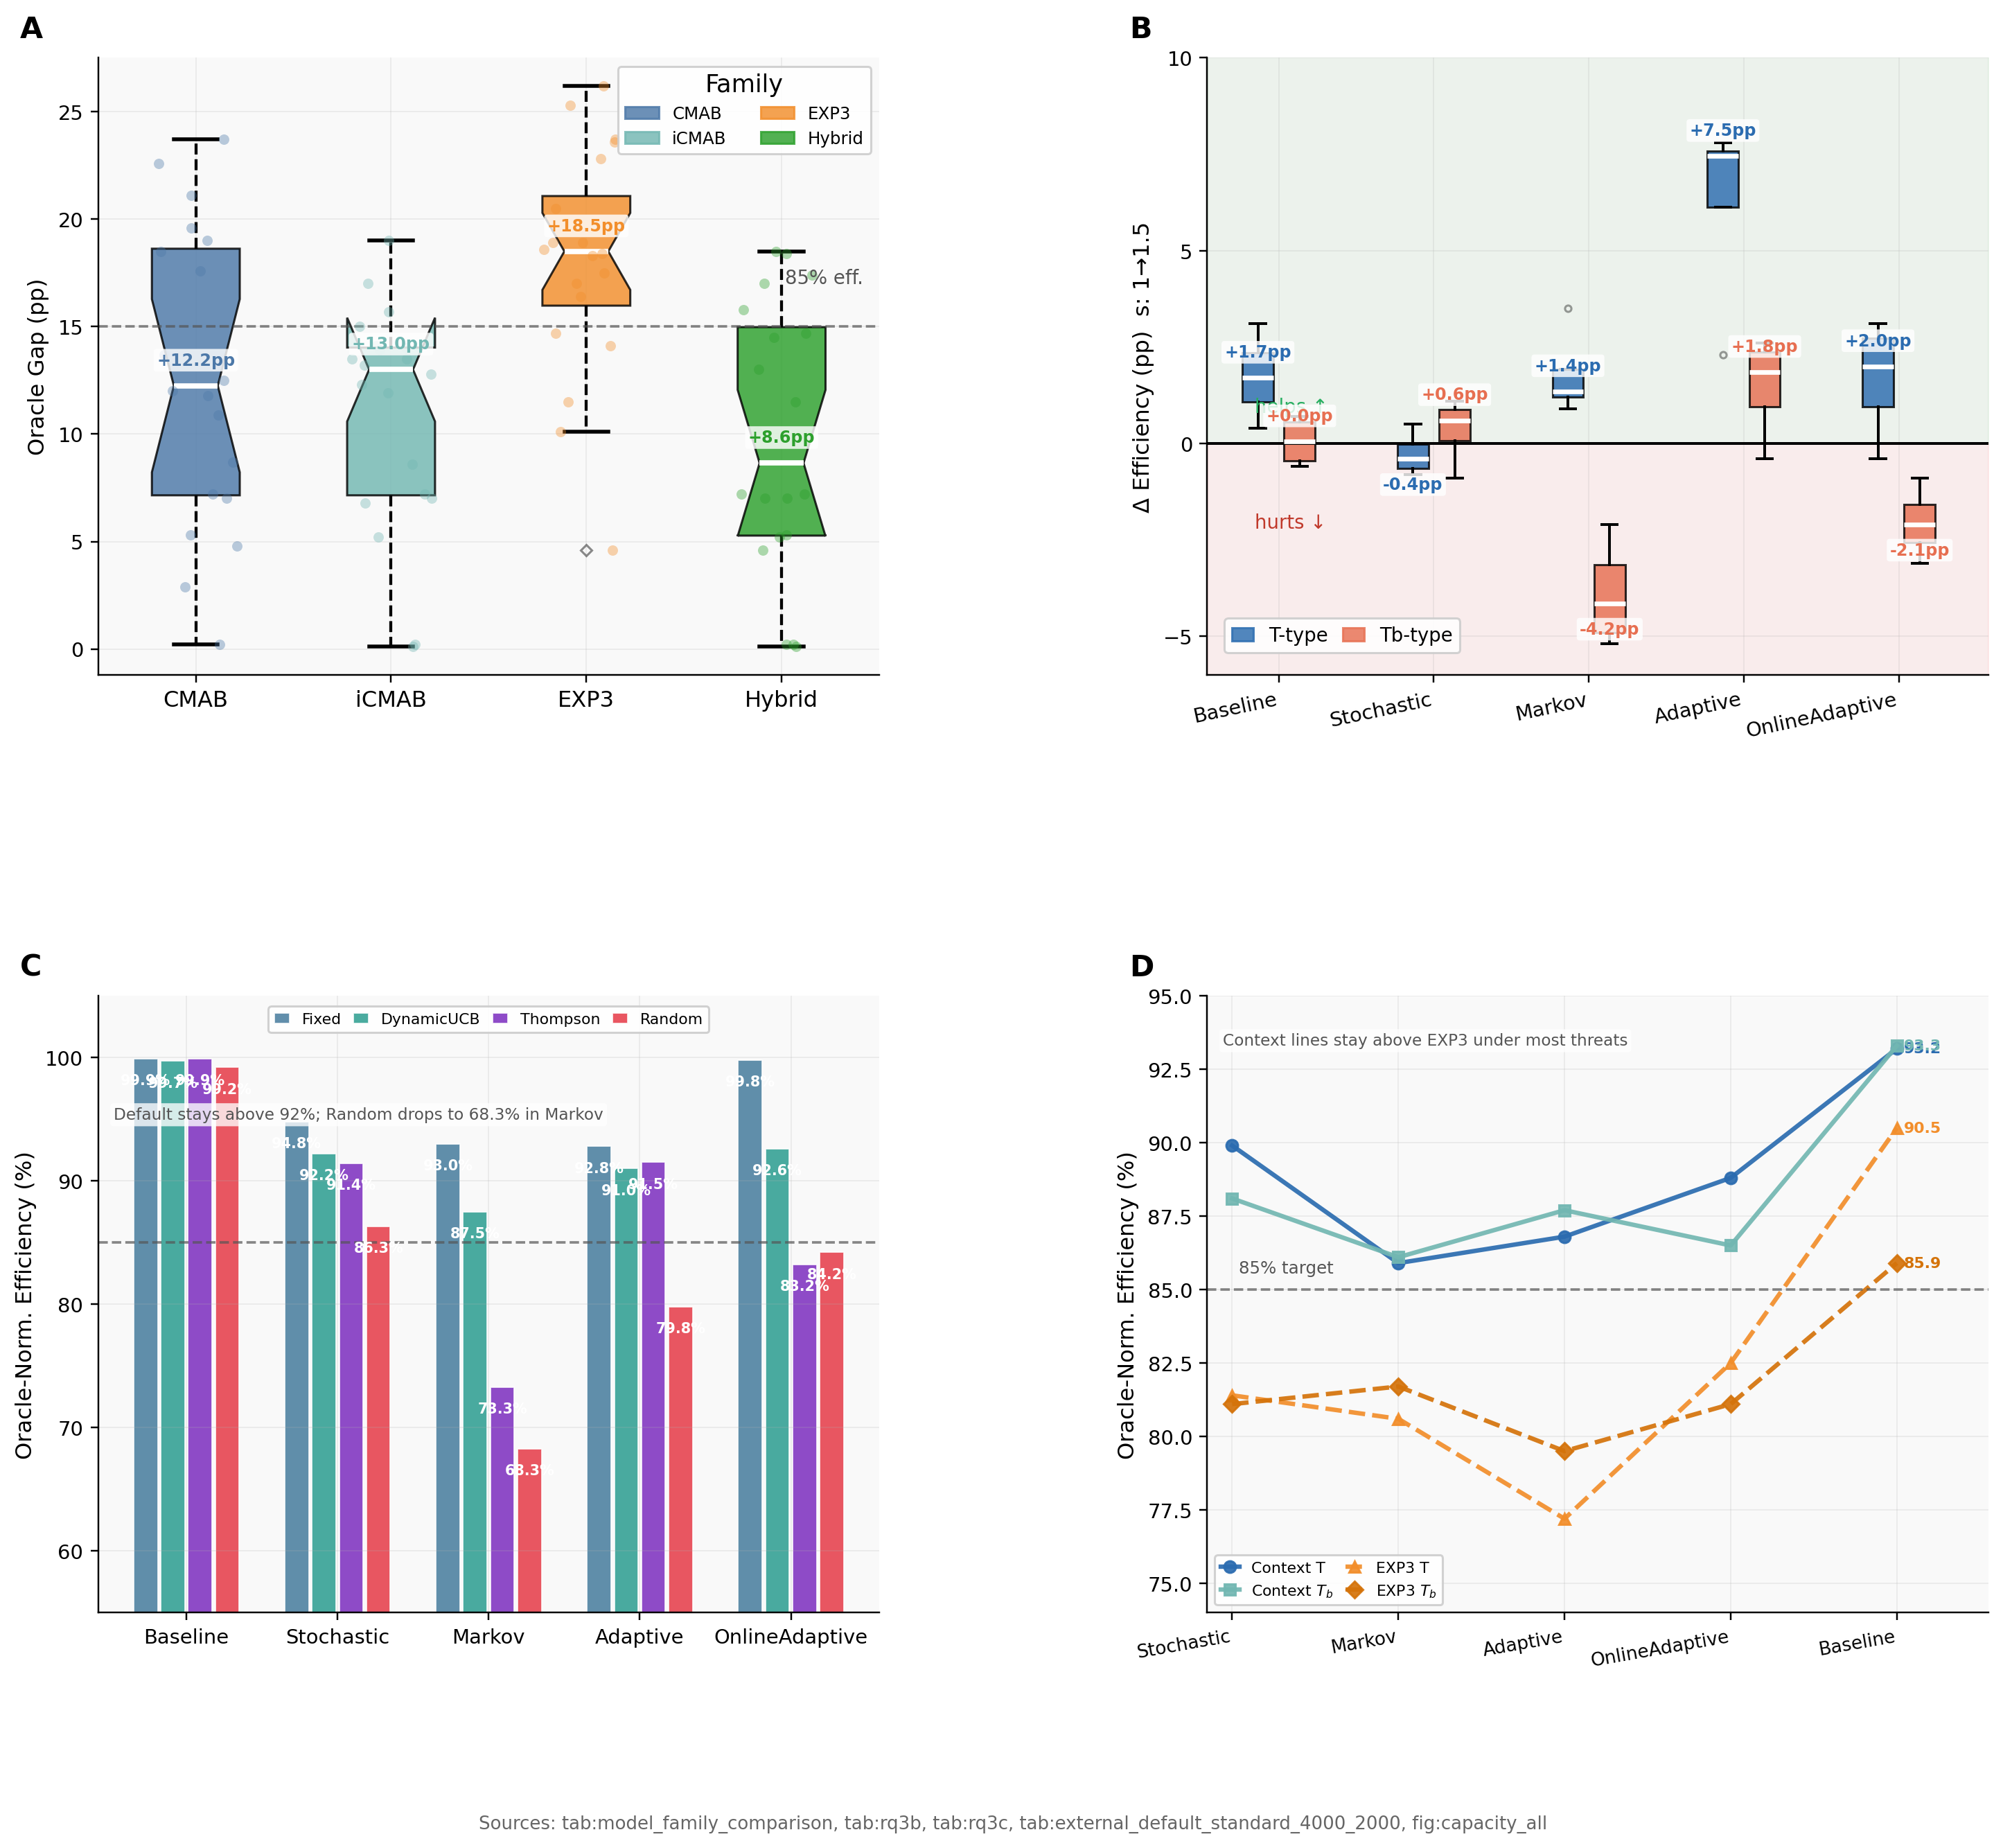
\includegraphics[width=0.98\textwidth]{figures/icnp/ICNP-CODE-024_g8_advanced_4panel_grouped_full_figure.png}
\caption{Advanced synthesis diagnostic. This grouped figure summarizes oracle-gap distributions, capacity-paradox behavior, allocator efficiency, and cross-testbed efficiency/oracle-gap trends.}
\label{fig:appendix_g8_advanced_synthesis}
\end{figure*}

\begin{figure*}[t]
\centering
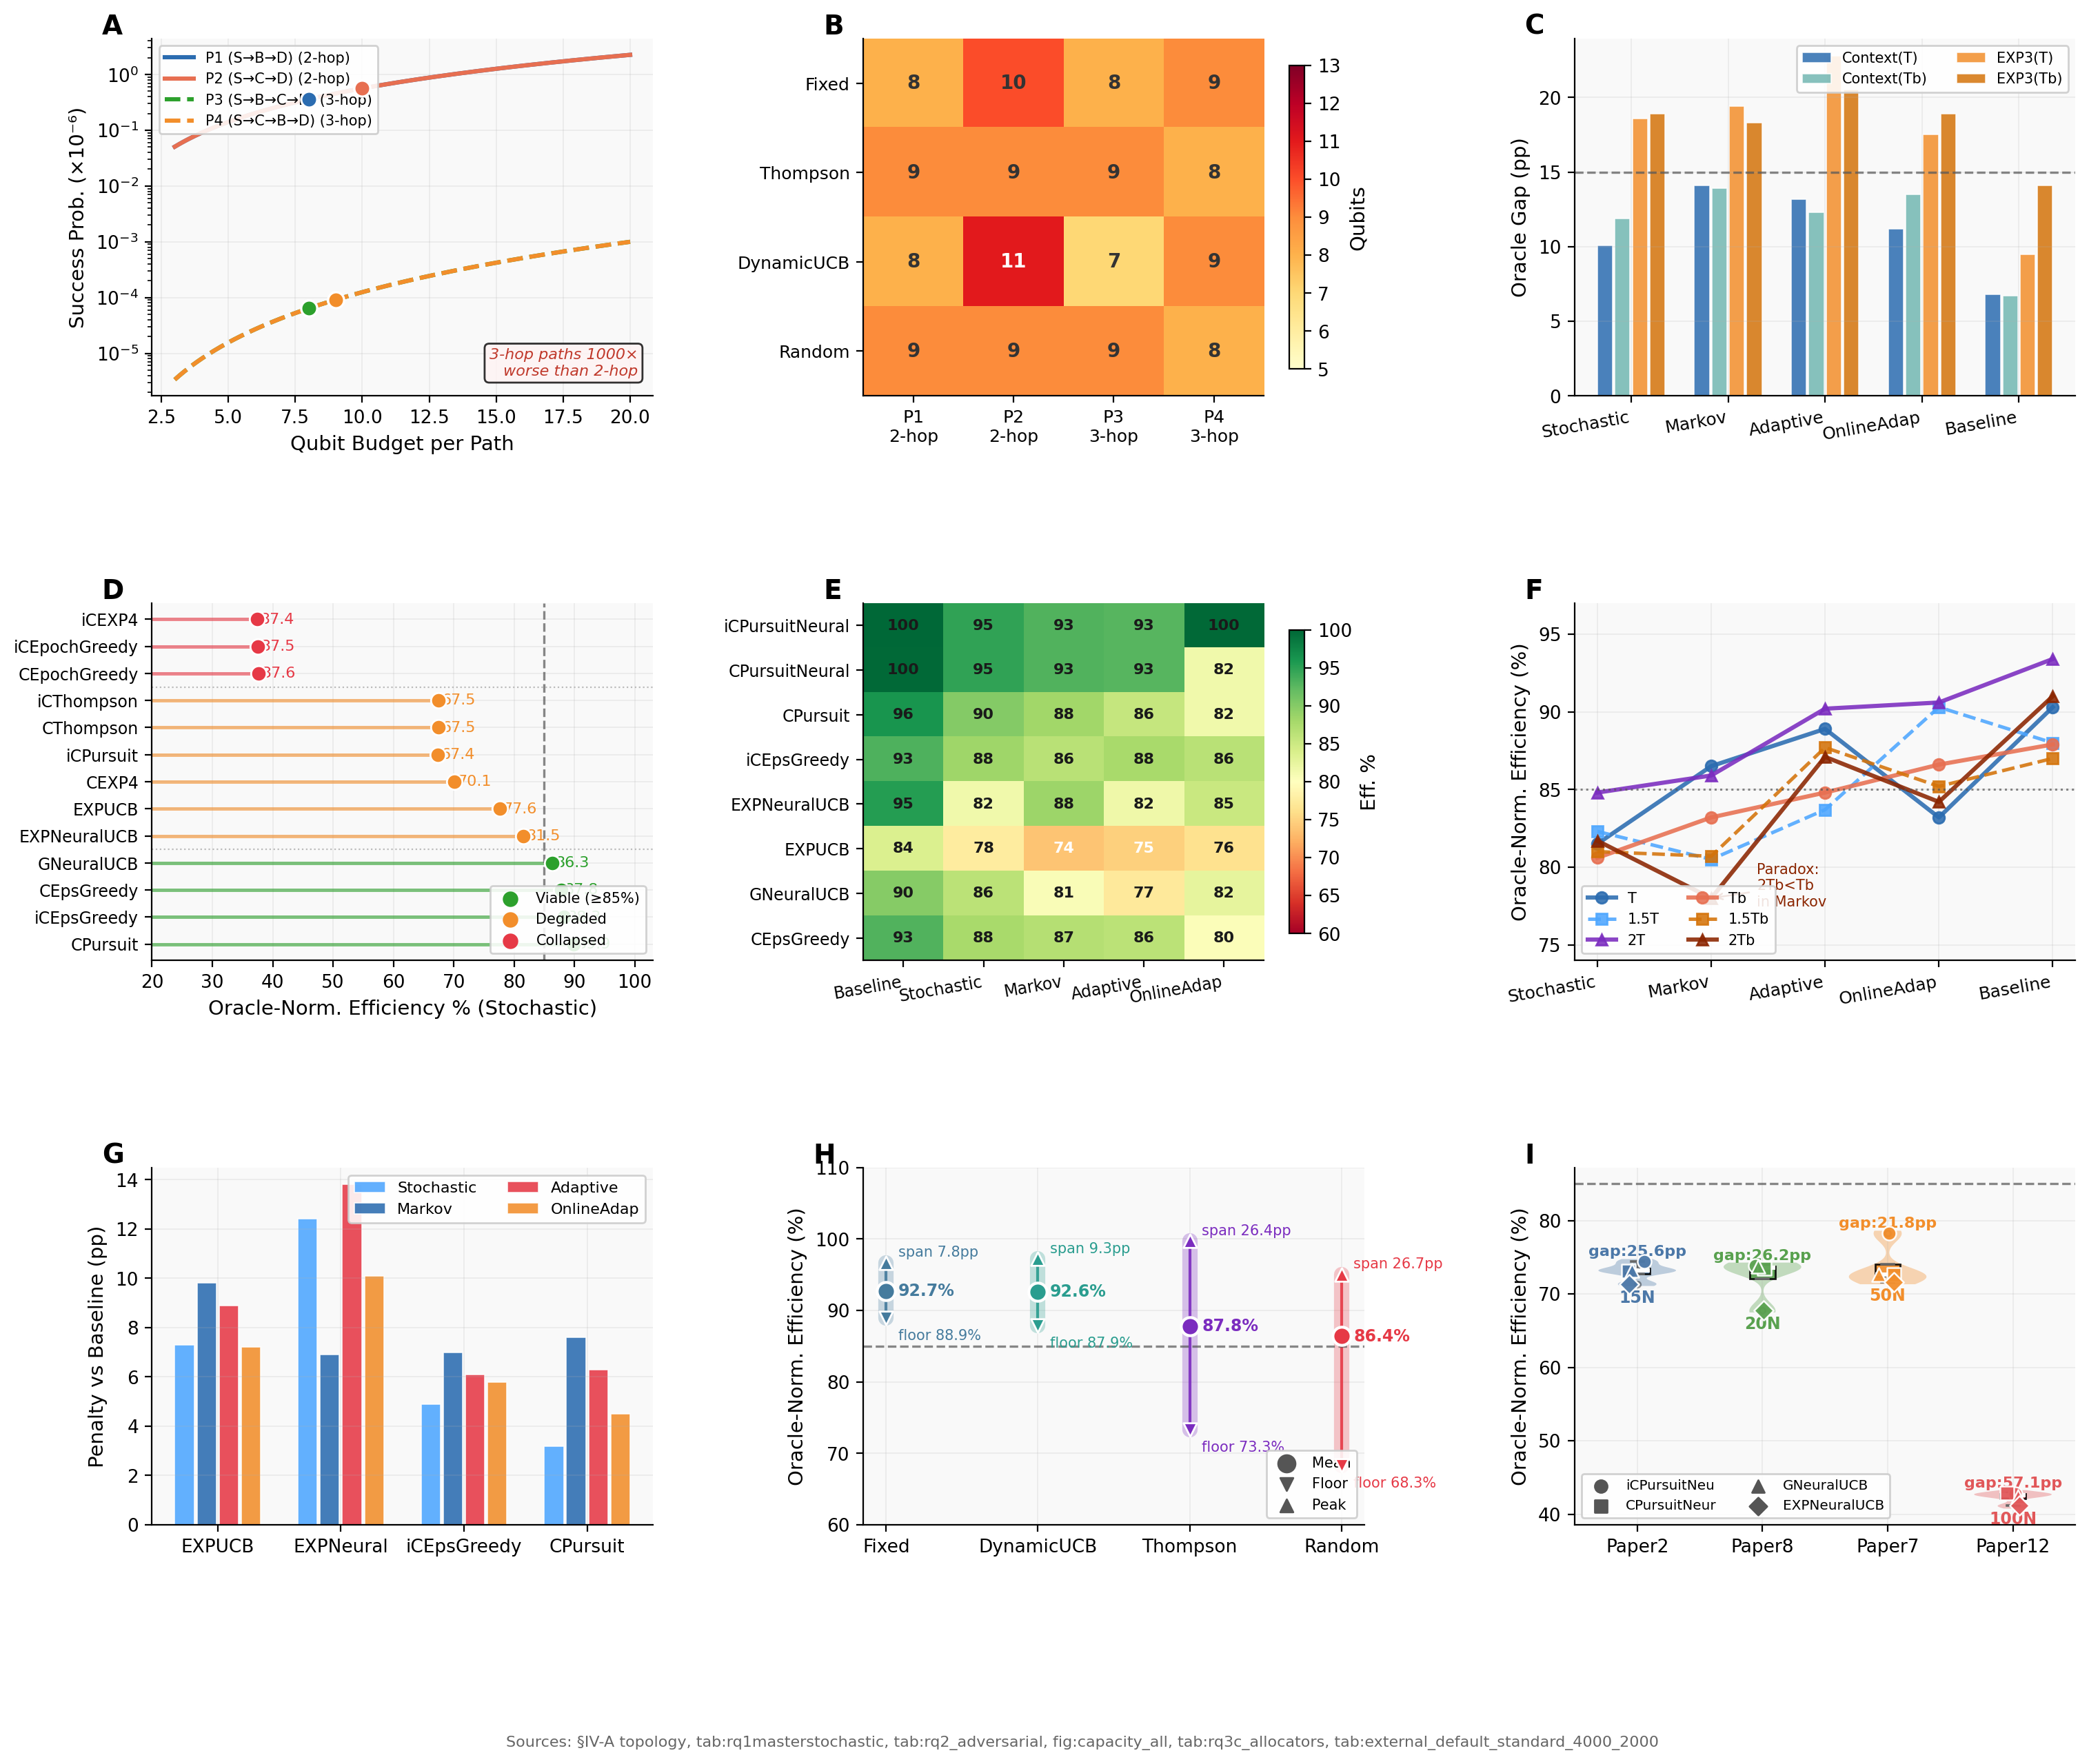
\includegraphics[width=0.98\textwidth]{figures/icnp/ICNP-CODE-029_g9_network_gap_analysis_grouped_full_figure.png}
\caption{Network-gap diagnostic suite. This grouped figure provides additional detail on path/fidelity structure, allocator budgets, threat escalation, capacity sensitivity, scenario penalties, allocator risk, and cross-testbed behavior.}
\label{fig:appendix_g9_network_gap_analysis}
\end{figure*}

\begin{figure}[t]
\centering
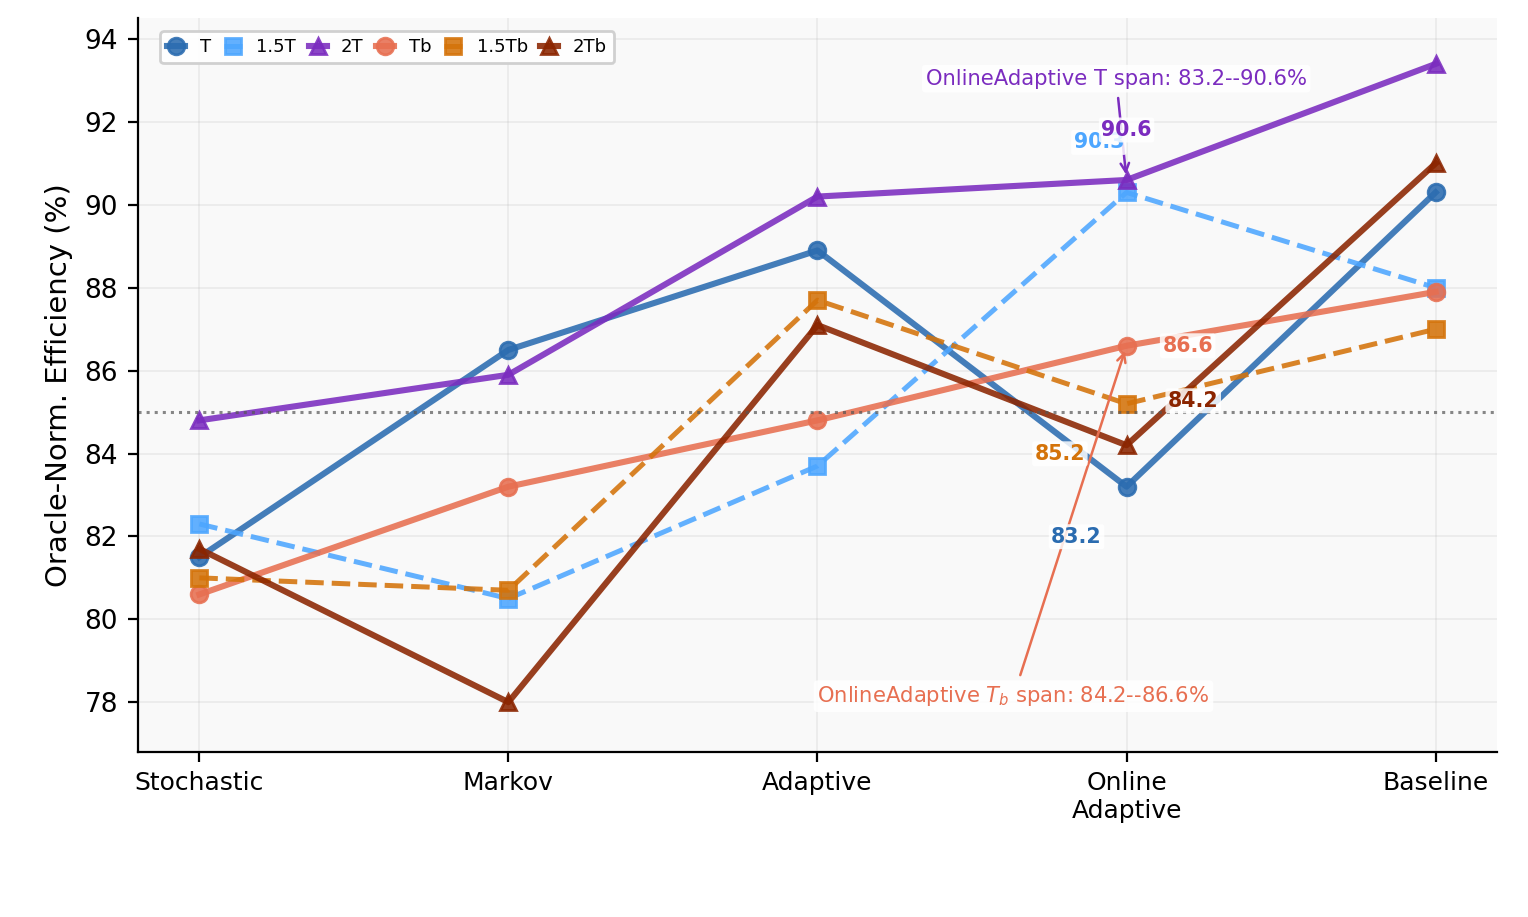
\includegraphics[width=\columnwidth]{figures/icnp/ICNP-CODE-035_g9_network_gap_analysis_panel_f_capacity_paradox_all_6_replay_configs_sc.png}
\caption{Detailed capacity-paradox diagnostic across replay configurations and scenarios. This figure supports the compact main-body capacity-paradox result in \Cref{fig:capacity_paradox}.}
\label{fig:appendix_capacity_paradox_all_configs}
\end{figure}

\begin{figure}[t]
\centering
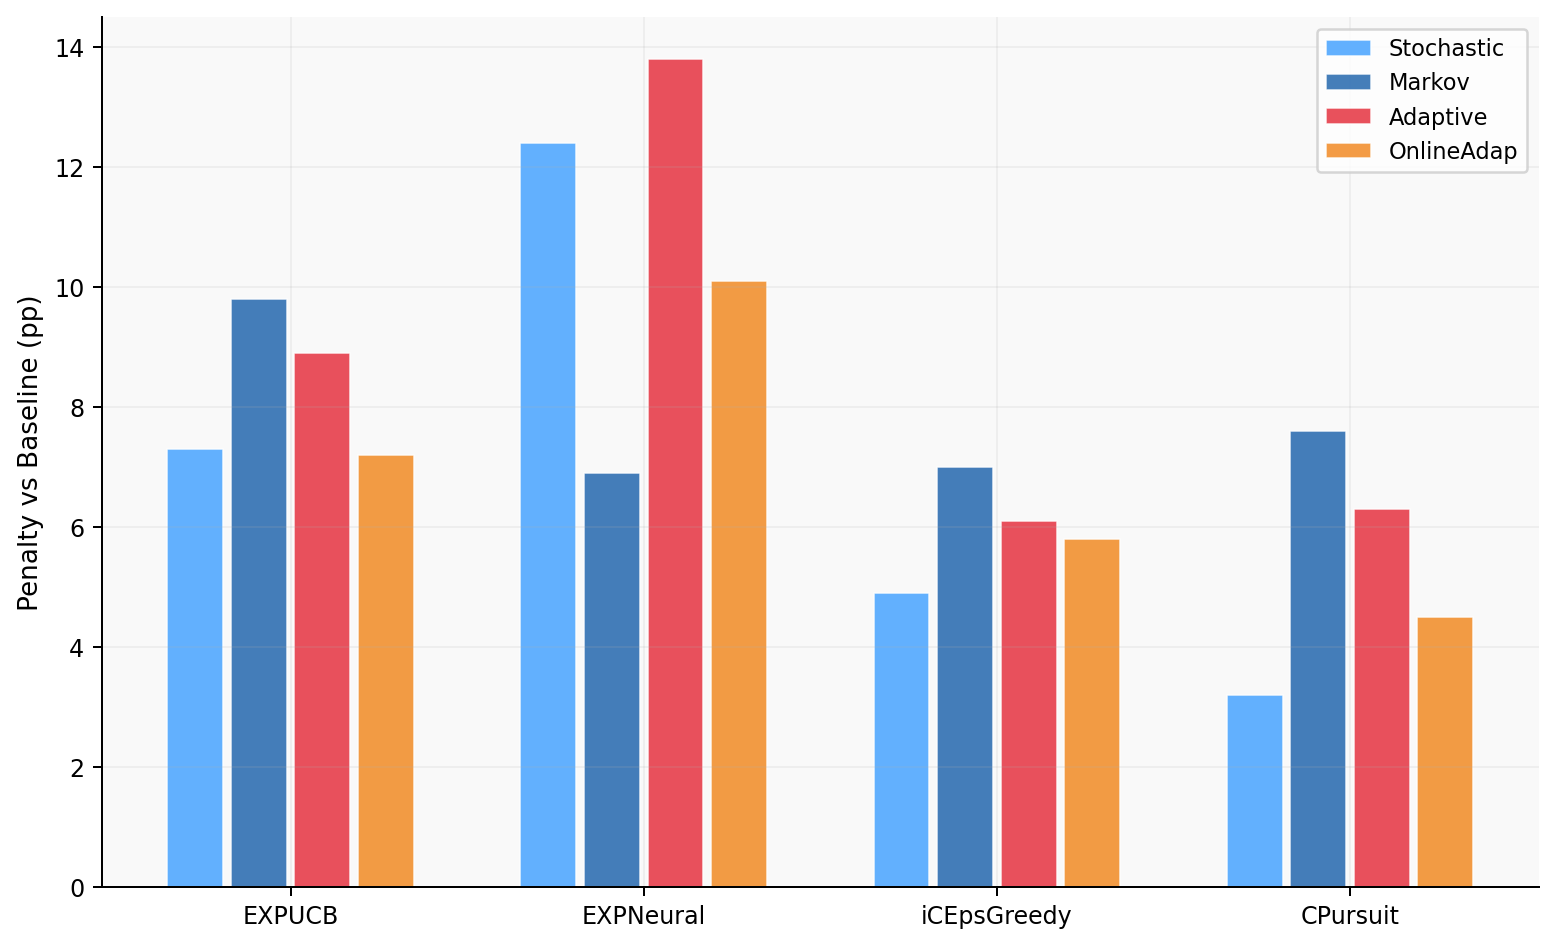
\includegraphics[width=\columnwidth]{figures/icnp/ICNP-CODE-036_g9_network_gap_analysis_panel_g_scenario_penalty_vs_baseline_by_algorith.png}
\caption{Scenario-penalty diagnostic by algorithm and threat. This figure provides additional support for the robustness-floor analysis in \Cref{fig:robustness_floor}.}
\label{fig:appendix_scenario_penalty}
\end{figure}

\begin{figure}[t]
\centering
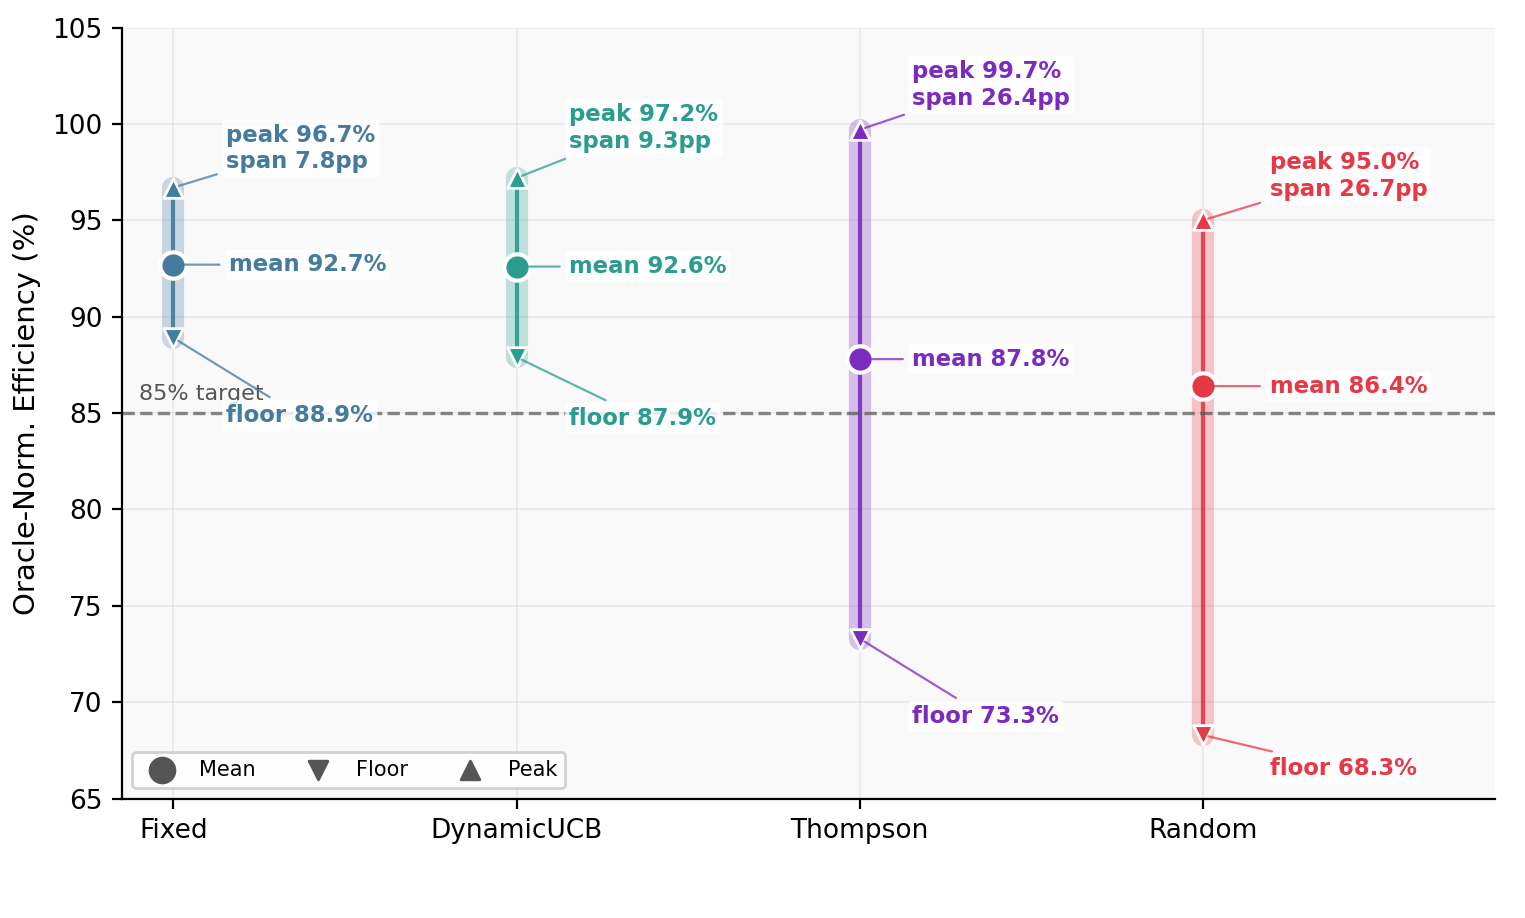
\includegraphics[width=\columnwidth]{figures/icnp/ICNP-CODE-037_g9_network_gap_analysis_panel_h_allocator_risk_floor_mean_peak_icpursuit.png}
\caption{Allocator-risk diagnostic for the pursuit-neural family. This figure supports the deployment guidance and allocator-risk conclusions in \Cref{fig:deployment_guidance}.}
\label{fig:appendix_allocator_risk}
\end{figure}

\begin{figure}[t]
\centering
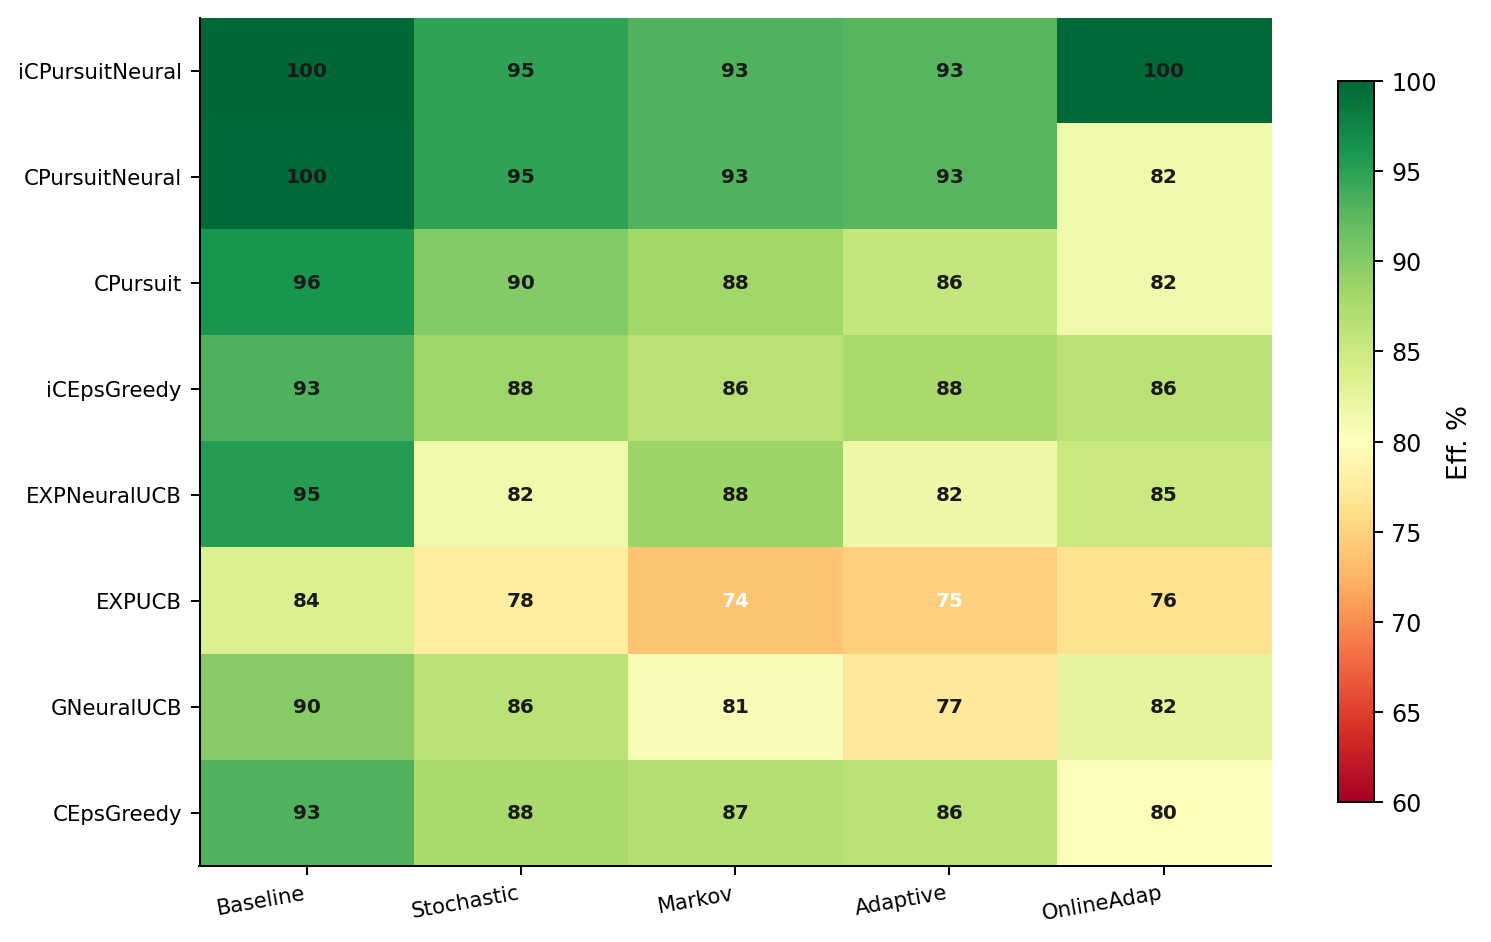
\includegraphics[width=\columnwidth]{figures/icnp/ICNP-CODE-034_g9_network_gap_analysis_panel_e_threat_escalation_heatmap_algo_scenario.png}
\caption{Threat-escalation heatmap diagnostic. This figure shows algorithm-by-scenario structure behind the compact main-body threat-robustness claims.}
\label{fig:appendix_threat_escalation_heatmap}
\end{figure}
